\chapter{Data Similarity and Introduction to Cluster Analysis}
\label{ch:similarity-clustering}

% ============================================================
%  PART I – SIMILARITY AND DISTANCE
% ============================================================

\section{Proximity: Similarity and Dissimilarity}
\label{sec:proximity}

Every Data Mining technique that involves comparing objects — from classification to clustering, from information retrieval to anomaly detection — relies on a fundamental concept: \textbf{proximity}, an umbrella term encompassing both \textit{similarity} and \textit{dissimilarity}.

\begin{definition}[Similarity]
\textbf{Similarity} is a numerical measure of how alike two data objects are. It is higher when objects are more alike, and typically falls in the range $[0, 1]$.
\end{definition}

\begin{definition}[Dissimilarity]
\textbf{Dissimilarity} is a numerical measure of how different two data objects are. It assumes its minimum value (often $0$) when objects are identical; the upper limit varies depending on the chosen measure.
\end{definition}

The relationship between the two is intuitive: low dissimilarity corresponds to high similarity. In practice, transformations such as $s = 1 - d$ or $s = e^{-d}$ convert distance into similarity.

\subsection{Proximity for a Single Attribute}

Before tackling the multi-dimensional case, it is useful to examine how proximity is defined for a single attribute depending on its type:

\begin{table}[htbp]
\centering
\small
\begin{tabularx}{\textwidth}{>{\bfseries\raggedright\arraybackslash}p{4.2cm} >{\raggedright\arraybackslash}X >{\raggedright\arraybackslash}X}
\toprule
Attribute Type & Dissimilarity & Similarity \\
\midrule
Nominal & $d = 0$ if $p = q$; \quad $d = 1$ otherwise & $s = 1$ if $p = q$; \quad $s = 0$ otherwise \\
\addlinespace[6pt]
Ordinal & $d = \dfrac{|p - q|}{n - 1}$ \newline {\scriptsize(values mapped to $0, \ldots, n-1$)} & $s = 1 - d$ \\
\addlinespace[6pt]
Interval / Ratio & $d = |p - q|$ & $s = -d$, \quad $s = \dfrac{1}{1+d}$, \newline or $s = e^{-\alpha d}$ \\
\bottomrule
\end{tabularx}
\caption{Proximity measures for a single attribute by data type.}
\label{tab:proximity-one-attr}
\end{table}

% ============================================================
\section{Euclidean Distance and Metric Properties}
\label{sec:euclidean}

When data objects are points in $\mathbb{R}^n$, the most natural distance measure is the \textbf{Euclidean distance}.

\begin{definition}[Euclidean Distance]
For two points $\mathbf{x} = (x_1, \ldots, x_n)$ and $\mathbf{y} = (y_1, \ldots, y_n)$ in $\mathbb{R}^n$, the \textbf{Euclidean distance} ($L_2$ norm) is:
\begin{equation}
  d(\mathbf{x}, \mathbf{y}) = \sqrt{\sum_{k=1}^{n} (x_k - y_k)^2}
  \label{eq:euclidean}
\end{equation}
\end{definition}

\begin{noteblock}{Standardization Required}
If attribute scales differ (e.g., one attribute in $[0,1]$ and another in $[0, 10{,}000]$), attributes with a larger range will dominate the distance computation. \textbf{Standardization} (subtract mean, divide by standard deviation) should be applied before computing Euclidean distances.
\end{noteblock}

\begin{example}[Euclidean Distance Matrix]
Consider four points in the plane:

\begin{center}
\begin{tabularx}{0.4\textwidth}{c c c}
\toprule
Point & $x$ & $y$ \\
\midrule
$p_1$ & 0 & 2 \\
$p_2$ & 2 & 0 \\
$p_3$ & 3 & 1 \\
$p_4$ & 5 & 1 \\
\bottomrule
\end{tabularx}
\end{center}

The resulting Euclidean distance matrix is:

\begin{center}
\begin{tabular}{c | c c c c}
\toprule
 & $p_1$ & $p_2$ & $p_3$ & $p_4$ \\
\midrule
$p_1$ & 0 & 2.828 & 3.162 & 5.099 \\
$p_2$ & 2.828 & 0 & 1.414 & 3.162 \\
$p_3$ & 3.162 & 1.414 & 0 & 2.000 \\
$p_4$ & 5.099 & 3.162 & 2.000 & 0 \\
\bottomrule
\end{tabular}
\end{center}
\end{example}

\subsection{Properties of a Metric}

A distance function $d(\mathbf{x}, \mathbf{y})$ satisfying the following three properties is called a \textbf{metric}:

\begin{enumerate}
  \item \textbf{Positive definiteness:} $d(\mathbf{x}, \mathbf{y}) \geq 0$ for all $\mathbf{x}, \mathbf{y}$, and $d(\mathbf{x}, \mathbf{y}) = 0$ if and only if $\mathbf{x} = \mathbf{y}$.
  \item \textbf{Symmetry:} $d(\mathbf{x}, \mathbf{y}) = d(\mathbf{y}, \mathbf{x})$ for all $\mathbf{x}, \mathbf{y}$.
  \item \textbf{Triangle inequality:} $d(\mathbf{x}, \mathbf{z}) \leq d(\mathbf{x}, \mathbf{y}) + d(\mathbf{y}, \mathbf{z})$ for all $\mathbf{x}, \mathbf{y}, \mathbf{z}$.
\end{enumerate}

Similarly, a similarity function $s(\mathbf{x}, \mathbf{y})$ satisfies:
\begin{enumerate}
  \item $s(\mathbf{x}, \mathbf{y}) = 1$ (maximum similarity) if and only if $\mathbf{x} = \mathbf{y}$.
  \item $s(\mathbf{x}, \mathbf{y}) = s(\mathbf{y}, \mathbf{x})$ for all $\mathbf{x}, \mathbf{y}$ (symmetry).
\end{enumerate}

% ============================================================
\section{Minkowski Distance: A Family of Metrics}
\label{sec:minkowski}

The Euclidean distance is a special case of a more general family, the \textbf{Minkowski distance}.

\begin{definition}[Minkowski Distance]
For two points $\mathbf{x}, \mathbf{y} \in \mathbb{R}^n$ and parameter $r \geq 1$, the \textbf{Minkowski distance} ($L_r$ norm) is:
\begin{equation}
  d(\mathbf{x}, \mathbf{y}) = \left( \sum_{k=1}^{n} |x_k - y_k|^r \right)^{1/r}
  \label{eq:minkowski}
\end{equation}
\end{definition}

The parameter $r$ controls the ``shape'' of the unit ball associated with the norm:

\begin{figure}[htbp]
\centering
\resizebox{0.92\linewidth}{!}{%
\begin{tikzpicture}[
  box/.style={rectangle, rounded corners=5pt, draw=blue!60!black, fill=blue!7, thick,
              minimum width=3.6cm, minimum height=2.2cm, align=center, font=\small},
  arr/.style={-Stealth, thick, gray!70}
]
  \node[box] (l1) at (0, 0) {
    $r = 1$ \\[4pt]
    \textbf{$L_1$ Norm} \\[2pt]
    \scriptsize Manhattan, Taxicab \\
    \scriptsize City-block, Hamming
  };
  \node[box, draw=green!60!black, fill=green!7] (l2) at (5.5, 0) {
    $r = 2$ \\[4pt]
    \textbf{$L_2$ Norm} \\[2pt]
    \scriptsize Euclidean Distance \\
    \scriptsize (standard case)
  };
  \node[box, draw=orange!70!black, fill=orange!8] (linf) at (11, 0) {
    $r \to \infty$ \\[4pt]
    \textbf{$L_\infty$ Norm} \\[2pt]
    \scriptsize Supremum / Chebyshev \\
    \scriptsize $\max_k |x_k - y_k|$
  };
  \draw[arr] (l1.east) -- (l2.west) node[midway, above, font=\scriptsize] {smoother};
  \draw[arr] (l2.east) -- (linf.west) node[midway, above, font=\scriptsize] {increasing $r$};
  \node[font=\scriptsize, below=0.25cm of l1] {$\sum_k |x_k - y_k|$};
  \node[font=\scriptsize, below=0.25cm of l2] {$\sqrt{\sum_k (x_k-y_k)^2}$};
  \node[font=\scriptsize, below=0.25cm of linf] {$\max_k |x_k - y_k|$};
\end{tikzpicture}%
}
\caption{The Minkowski family of norms as the parameter $r$ varies.}
\label{fig:minkowski-family}
\end{figure}

\begin{example}[Comparison of $L_1$, $L_2$, and $L_\infty$ distances]
Using the same four points from the previous example:

\begin{center}
\small
\begin{tabular}{c | c c c c}
\toprule
$L_1$ & $p_1$ & $p_2$ & $p_3$ & $p_4$ \\
\midrule
$p_1$ & 0 & 4 & 4 & 6 \\
$p_2$ & 4 & 0 & 2 & 4 \\
$p_3$ & 4 & 2 & 0 & 2 \\
$p_4$ & 6 & 4 & 2 & 0 \\
\bottomrule
\end{tabular}
\hspace{1cm}
\begin{tabular}{c | c c c c}
\toprule
$L_\infty$ & $p_1$ & $p_2$ & $p_3$ & $p_4$ \\
\midrule
$p_1$ & 0 & 2 & 3 & 5 \\
$p_2$ & 2 & 0 & 1 & 3 \\
$p_3$ & 3 & 1 & 0 & 2 \\
$p_4$ & 5 & 3 & 2 & 0 \\
\bottomrule
\end{tabular}
\end{center}

Under $L_1$: $d(p_1, p_2) = |0-2|+|2-0| = 4$. Under $L_\infty$: $d(p_1, p_2) = \max(|0-2|, |2-0|) = 2$.
\end{example}

The $L_1$ norm is especially useful for high-dimensional sparse data. The \textbf{Hamming distance} — the number of differing bits between two binary vectors — is a special case of the $L_1$ norm.

% ============================================================
\section{Similarity Between Binary Data}
\label{sec:binary-similarity}

When attributes are \textbf{binary} (present/absent, true/false), Euclidean distance loses semantic meaning. Instead, we reason in terms of \textit{matches} and \textit{mismatches}.

Given two objects $p$ and $q$ with binary attributes, we define the following \textbf{contingency table}:

\begin{center}
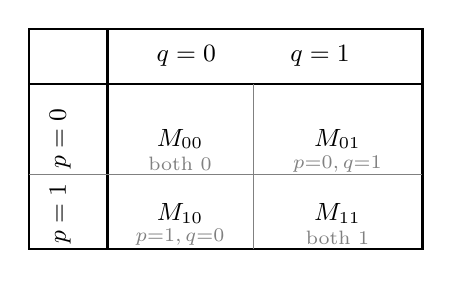
\begin{tikzpicture}[font=\small]
  \draw[thick] (-0.5, -1.8) rectangle (4.5, 1.0);
  \node at (1.5, 0.65) {\textbf{$q=0$}};
  \node at (3.2, 0.65) {\textbf{$q=1$}};
  \node at (-0.1, -0.4) [rotate=90] {\textbf{$p=0$}};
  \node at (-0.1, -1.35) [rotate=90] {\textbf{$p=1$}};
  \draw[thick] (-0.5, 0.3) -- (4.5, 0.3);
  \draw[thick] (0.5, -1.8) -- (0.5, 1.0);
  \draw[gray] (2.35, -1.8) -- (2.35, 0.3);
  \draw[gray] (-0.5, -0.85) -- (4.5, -0.85);
  \node at (1.42, -0.4)  {$M_{00}$};
  \node at (3.42, -0.4)  {$M_{01}$};
  \node at (1.42, -1.35) {$M_{10}$};
  \node at (3.42, -1.35) {$M_{11}$};
  \node[font=\scriptsize, text=gray] at (1.42, -0.72) {both 0};
  \node[font=\scriptsize, text=gray] at (3.42, -0.72) {$p{=}0, q{=}1$};
  \node[font=\scriptsize, text=gray] at (1.42, -1.65) {$p{=}1, q{=}0$};
  \node[font=\scriptsize, text=gray] at (3.42, -1.65) {both 1};
\end{tikzpicture}
\end{center}

\begin{definition}[Simple Matching Coefficient — SMC]
\begin{equation}
  \mathrm{SMC}(p, q) = \frac{M_{11} + M_{00}}{M_{01} + M_{10} + M_{11} + M_{00}}
  \label{eq:smc}
\end{equation}
Counts both $1$-$1$ matches and $0$-$0$ matches.
\end{definition}

\begin{definition}[Jaccard Coefficient]
\begin{equation}
  J(p, q) = \frac{M_{11}}{M_{01} + M_{10} + M_{11}}
  \label{eq:jaccard}
\end{equation}
Ignores $0$-$0$ matches: suitable when attribute absence is not informative (e.g., market-basket data, disease occurrence).
\end{definition}

\begin{example}[SMC vs.\ Jaccard]
Let:
\[
  p = [1, 0, 0, 0, 0, 0, 0, 0, 0, 0], \quad q = [0, 0, 0, 0, 0, 0, 1, 0, 0, 1]
\]
\begin{itemize}
  \item $M_{11} = 0$, $M_{10} = 1$, $M_{01} = 2$, $M_{00} = 7$
\end{itemize}
\[
  \mathrm{SMC} = \frac{0+7}{2+1+0+7} = 0.7, \qquad J = \frac{0}{2+1+0} = 0
\]
SMC is high because of the 7 shared zeros. Jaccard is 0 because there are no co-occurrences of 1. For market-basket data, Jaccard is the appropriate choice.
\end{example}

% ============================================================
\section{Cosine Similarity}
\label{sec:cosine}

In document data (word frequency or TF-IDF vectors), vectors are typically high-dimensional and sparse. Euclidean distance is sensitive to document length; \textbf{cosine similarity} normalizes by vector magnitude and measures only the angle between vectors.

\begin{definition}[Cosine Similarity]
For two vectors $\mathbf{d}_1, \mathbf{d}_2 \in \mathbb{R}^n$:
\begin{equation}
  \cos(\mathbf{d}_1, \mathbf{d}_2) = \frac{\mathbf{d}_1 \cdot \mathbf{d}_2}{\|\mathbf{d}_1\| \, \|\mathbf{d}_2\|}
  \label{eq:cosine}
\end{equation}
where $\mathbf{d}_1 \cdot \mathbf{d}_2 = \sum_k d_{1k} d_{2k}$ and $\|\mathbf{d}\| = \sqrt{\sum_k d_k^2}$.
\end{definition}

The value lies in $[-1, 1]$; for non-negative vectors (such as word frequencies), the range is $[0, 1]$: $1$ means identical directions, $0$ means orthogonal vectors.

\begin{example}[Cosine Similarity on Documents]
\begin{align*}
  \mathbf{d}_1 &= [3, 2, 0, 5, 0, 0, 0, 2, 0, 0] \\
  \mathbf{d}_2 &= [1, 0, 0, 0, 0, 0, 0, 1, 0, 2]
\end{align*}
\[
  \mathbf{d}_1 \cdot \mathbf{d}_2 = 3{\cdot}1 + 2{\cdot}1 = 5
\]
\[
  \|\mathbf{d}_1\| = \sqrt{9+4+25+4} = \sqrt{42} \approx 6.481, \quad
  \|\mathbf{d}_2\| = \sqrt{1+1+4} = \sqrt{6} \approx 2.449
\]
\[
  \cos(\mathbf{d}_1, \mathbf{d}_2) \approx 0.315
\]
The documents share about 31.5\% of ``direction'', regardless of their different lengths.
\end{example}

\subsection{Weighted Similarity}

When attributes have different importance, a \textbf{weighted similarity} can be defined with non-negative weights $w_k$ summing to 1:
\begin{equation}
  s_w(\mathbf{x}, \mathbf{y}) = \frac{\sum_{k=1}^{n} w_k \cdot d_k \cdot s_k(x_k, y_k)}{\sum_{k=1}^{n} w_k \cdot d_k}
\end{equation}

% ============================================================
\section{Correlation}
\label{sec:correlation}

\textbf{Pearson correlation} measures the \textit{linear} relationship between two variables (or between two objects viewed as attribute vectors). It is computed by standardizing the vectors and taking their dot product:
\begin{equation}
  \mathrm{corr}(p, q) = \frac{\sum_{k=1}^{n}(p_k - \bar{p})(q_k - \bar{q})}{(n-1)\,\sigma_p\,\sigma_q}
  \label{eq:pearson}
\end{equation}
The result lies in $[-1, 1]$: $+1$ perfect positive correlation, $0$ no linear relationship, $-1$ perfect negative correlation.

% ============================================================
\section{Information-Based Measures: Entropy and Mutual Information}
\label{sec:entropy}

Information-theoretic measures allow quantifying proximity between categorical or continuous variables in a non-linear way, going beyond simple value-by-value comparisons.

\subsection{Entropy}

The information content of an event is inversely proportional to its probability: a certain event carries no information; a rare event carries much.

\begin{definition}[Shannon Entropy]
For a discrete variable $X$ with $n$ possible values $x_1, \ldots, x_n$ and probabilities $p_1, \ldots, p_n$:
\begin{equation}
  H(X) = -\sum_{i=1}^{n} p_i \log_2 p_i
  \label{eq:entropy}
\end{equation}
Entropy is measured in \textbf{bits} and lies in $[0, \log_2 n]$.
\end{definition}

Boundary cases:
\begin{itemize}
  \item If one probability equals 1 (certain event): $H = 0$ — maximum certainty, zero information.
  \item If all values are equally likely ($p_i = 1/n$): $H = \log_2 n$ — maximum uncertainty.
\end{itemize}

\begin{example}[Fair vs.\ Biased Coin]
For a coin with probability $p$ of heads and $q = 1 - p$ of tails:
\[
  H = -p \log_2 p - q \log_2 q
\]
With $p = 0.5$ (fair coin): $H = 1$ bit. With $p = 1$ (biased): $H = 0$ bits.
\end{example}

\subsection{Mutual Information}

\textbf{Mutual Information} (MI) quantifies how much information variable $X$ provides about variable $Y$:

\begin{definition}[Mutual Information]
\begin{equation}
  I(X; Y) = H(X) + H(Y) - H(X, Y)
  \label{eq:mutual-info}
\end{equation}
where $H(X,Y) = -\sum_i \sum_j p_{ij} \log_2 p_{ij}$ is the joint entropy.
\end{definition}

$I(X;Y) = 0$ if and only if $X$ and $Y$ are independent. Unlike Pearson correlation, MI captures \textit{non-linear} dependencies.

\begin{example}[Mutual Information: Student Status and Grade]
For a class of 100 students with variables \textit{Student Status} (Undergraduate/Graduate) and \textit{Grade} (A/B/C):

\begin{center}
\small
\begin{tabularx}{0.85\linewidth}{l r r r}
\toprule
& \multicolumn{2}{c}{\textbf{Status}} & \\
\textbf{Grade} & Undergrad & Grad & Total \\
\midrule
A & 5 & 30 & 35 \\
B & 30 & 20 & 50 \\
C & 10 & 5  & 15 \\
\midrule
Total & 45 & 55 & 100 \\
\bottomrule
\end{tabularx}
\end{center}

$H(\text{Status}) \approx 0.993$ bit, \quad $H(\text{Grade}) \approx 1.441$ bit, \quad $H(\text{Status, Grade}) \approx 2.271$ bit
\[
  I(\text{Status}; \text{Grade}) = 0.993 + 1.441 - 2.271 \approx \mathbf{0.163} \text{ bit}
\]
\end{example}

% ============================================================
%  PART II – CLUSTER ANALYSIS
% ============================================================

\section{What is Cluster Analysis?}
\label{sec:cluster-analysis}

\begin{definition}[Cluster Analysis]
\textbf{Cluster analysis} (or \textbf{clustering}) is the process of grouping a set of data objects into \textbf{clusters} such that:
\begin{itemize}
  \item objects \textit{within} the same cluster are as similar as possible (\textit{high intra-cluster cohesion});
  \item objects in \textit{different} clusters are as dissimilar as possible (\textit{high inter-cluster separation}).
\end{itemize}
\end{definition}

\begin{figure}[htbp]
\centering
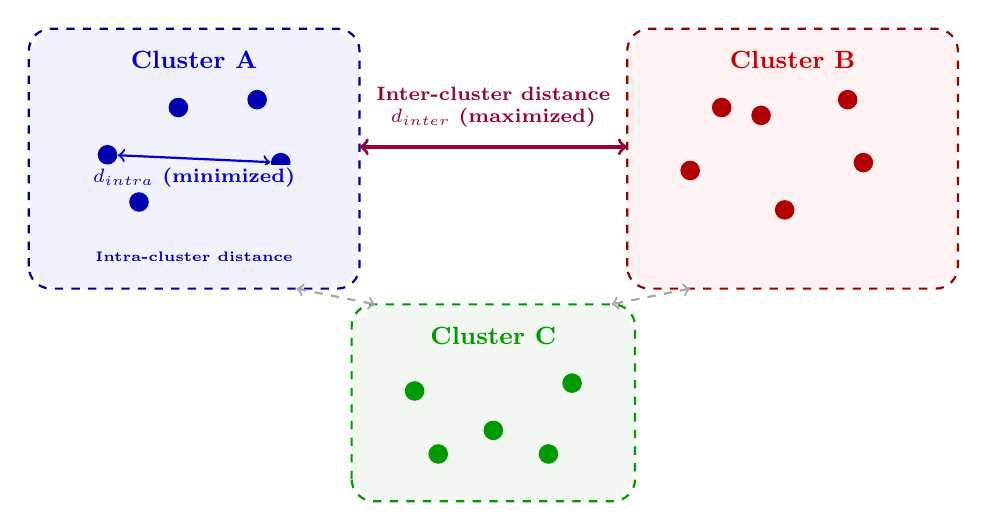
\begin{tikzpicture}[
  dotA/.style={circle, fill=blue!70!black, inner sep=2.5pt},
  dotB/.style={circle, fill=red!70!black, inner sep=2.5pt},
  dotC/.style={circle, fill=green!60!black, inner sep=2.5pt},
  clusterbox/.style={dashed, thick, rounded corners=8pt}
]
  % Cluster A (left) - width 4.2cm
  \fill[blue!5, rounded corners=12pt] (0.0, 0.6) rectangle (4.2, 3.9);
  \draw[blue!60!black, clusterbox] (0.0, 0.6) rectangle (4.2, 3.9);
  \node[font=\small\bfseries, text=blue!80!black] at (2.1, 3.5) {Cluster A};
  
  \node[dotA] (a1) at (1.0, 2.3) {};
  \node[dotA] (a2) at (1.9, 2.9) {};
  \node[dotA] (a3) at (3.2, 2.2) {};
  \node[dotA] at (1.4, 1.7) {};
  \node[dotA] at (2.9, 3.0) {};
  
  % Intra-cluster distance inside Cluster A
  \draw[<->, thick, blue!85!black] (a1) -- (a3)
    node[midway, below=2pt, font=\scriptsize\bfseries, fill=blue!5, inner sep=1pt] {$d_{\text{intra}}$ (minimized)};
  \node[font=\tiny\bfseries, text=blue!75!black, align=center] at (2.1, 1.0) {Intra-cluster distance};

  % Cluster B (right) - width 4.2cm
  \fill[red!5, rounded corners=12pt] (7.6, 0.6) rectangle (11.8, 3.9);
  \draw[red!60!black, clusterbox] (7.6, 0.6) rectangle (11.8, 3.9);
  \node[font=\small\bfseries, text=red!80!black] at (9.7, 3.5) {Cluster B};
  
  \node[dotB] at (8.4, 2.1) {};
  \node[dotB] at (9.3, 2.8) {};
  \node[dotB] at (10.6, 2.2) {};
  \node[dotB] at (8.8, 2.9) {};
  \node[dotB] at (10.4, 3.0) {};
  \node[dotB] at (9.6, 1.6) {};

  % Inter-cluster distance between Cluster A and Cluster B
  \draw[<->, very thick, purple!80!black] (4.2, 2.4) -- (7.6, 2.4)
    node[midway, above=3pt, font=\scriptsize\bfseries, align=center] {Inter-cluster distance\\$d_{\text{inter}}$ (maximized)};

  % Cluster C (bottom, centered between A and B)
  \fill[green!40!black!5, rounded corners=12pt] (4.1, -2.1) rectangle (7.7, 0.4);
  \draw[green!60!black, clusterbox] (4.1, -2.1) rectangle (7.7, 0.4);
  \node[font=\small\bfseries, text=green!60!black] at (5.9, 0.0) {Cluster C};

  \node[dotC] at (4.9, -0.7) {};
  \node[dotC] at (5.9, -1.2) {};
  \node[dotC] at (6.9, -0.6) {};
  \node[dotC] at (5.2, -1.5) {};
  \node[dotC] at (6.6, -1.5) {};

  % Dashed inter-cluster links to C
  \draw[<->, dashed, thick, gray!70] (3.4, 0.6) -- (4.4, 0.4);
  \draw[<->, dashed, thick, gray!70] (8.4, 0.6) -- (7.4, 0.4);
\end{tikzpicture}
\caption{Fundamental objective of clustering: maximize inter-cluster distances (separation) and minimize intra-cluster distances (cohesion).}
\label{fig:clustering-objective}
\end{figure}

Clustering is an \textbf{unsupervised learning} task: unlike classification, no predefined labels are available. The algorithm must autonomously discover latent structure in the data.

\subsection{Applications of Cluster Analysis}

Clustering is applied across a wide range of domains:

\begin{itemize}
  \item \textbf{Understanding:} group related documents by topic (IR), group genes with similar functionality (bioinformatics), group stocks with correlated price movements (finance).
  \item \textbf{Summarization and compression:} reduce large datasets by replacing each cluster with a representative (centroid or medoid).
  \item \textbf{Anomaly detection:} objects that do not belong to any cluster (or belong to very small clusters) are potential anomalies.
  \item \textbf{Spatial clustering:} discover geographic zones with similar environmental characteristics (e.g., precipitation patterns).
\end{itemize}

\subsection{What is NOT Cluster Analysis?}

\begin{itemize}
  \item \textbf{Simple segmentation:} dividing students into groups alphabetically is a partition, not clustering — groups are defined by an external rule, not by data similarity.
  \item \textbf{Query results:} retrieving all documents containing ``machine learning'' produces a set, not a clustering.
  \item \textbf{Supervised classification:} class labels are given a priori; clustering must discover them.
  \item \textbf{Association Analysis:} finds local relationships between items; clustering seeks global grouping structures.
\end{itemize}

% ============================================================
\section{Ambiguity and Subjectivity of Clusters}
\label{sec:cluster-ambiguity}

\begin{alertblock}{No Single Correct Answer}
The same point cloud can be validly interpreted as 2, 4, or 6 clusters depending on the scale of analysis, the chosen proximity measure, and the algorithm used. There is no ``objectively correct'' answer: clustering is always relative to the model and context.
\end{alertblock}

% ============================================================
\section{Taxonomy of Clusterings}
\label{sec:clustering-types}

A \textbf{clustering} is a collection of clusters that partitions or organizes the objects. Several orthogonal taxonomies exist.

\subsection{Partitional vs.\ Hierarchical Clustering}

\begin{figure}[htbp]
\centering
\resizebox{\linewidth}{!}{%
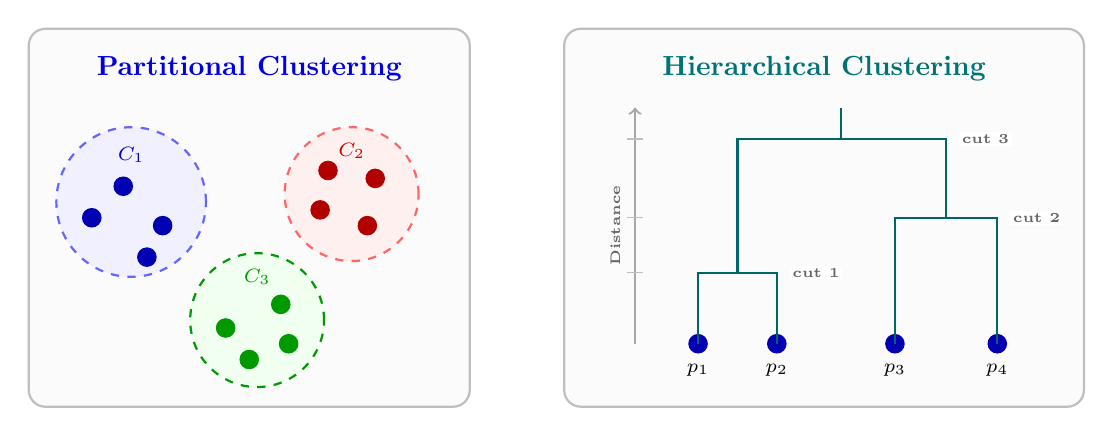
\begin{tikzpicture}[
  dot/.style={circle, fill=blue!70!black, inner sep=2.5pt},
  rdot/.style={circle, fill=red!70!black, inner sep=2.5pt},
  gdot/.style={circle, fill=green!60!black, inner sep=2.5pt},
  boxpanel/.style={draw=gray!50, thick, rounded corners=6pt, fill=gray!3}
]
  % === LEFT PANEL: Partitional Clustering ===
  \draw[boxpanel] (-0.2, -0.2) rectangle (5.4, 4.6);
  \node[font=\bfseries\normalsize, text=blue!90!black] at (2.6, 4.1) {Partitional Clustering};

  % Cluster 1
  \draw[blue!60, dashed, thick, fill=blue!6] (1.1, 2.4) circle(0.95);
  \node[font=\scriptsize\bfseries, text=blue!80!black] at (1.1, 3.0) {$C_1$};
  \node[dot] at (0.6, 2.2) {};
  \node[dot] at (1.0, 2.6) {};
  \node[dot] at (1.5, 2.1) {};
  \node[dot] at (1.3, 1.7) {};

  % Cluster 2
  \draw[red!60, dashed, thick, fill=red!6] (3.9, 2.5) circle(0.85);
  \node[font=\scriptsize\bfseries, text=red!80!black] at (3.9, 3.05) {$C_2$};
  \node[rdot] at (3.5, 2.3) {};
  \node[rdot] at (4.2, 2.7) {};
  \node[rdot] at (4.1, 2.1) {};
  \node[rdot] at (3.6, 2.8) {};

  % Cluster 3
  \draw[green!60!black, dashed, thick, fill=green!6] (2.7, 0.9) circle(0.85);
  \node[font=\scriptsize\bfseries, text=green!60!black] at (2.7, 1.45) {$C_3$};
  \node[gdot] at (2.3, 0.8) {};
  \node[gdot] at (3.0, 1.1) {};
  \node[gdot] at (2.6, 0.4) {};
  \node[gdot] at (3.1, 0.6) {};

  % === RIGHT PANEL: Hierarchical Clustering ===
  \draw[boxpanel] (6.6, -0.2) rectangle (13.2, 4.6);
  \node[font=\bfseries\normalsize, text=teal!90!black] at (9.9, 4.1) {Hierarchical Clustering};

  % Level / Distance axis
  \draw[->, thick, gray!70] (7.5, 0.6) -- (7.5, 3.6);
  \node[font=\tiny\bfseries, text=gray!80!black, rotate=90] at (7.25, 2.1) {Distance};
  \draw[gray!50] (7.4, 1.5) -- (7.6, 1.5);
  \draw[gray!50] (7.4, 2.2) -- (7.6, 2.2);
  \draw[gray!50] (7.4, 3.2) -- (7.6, 3.2);

  % Leaf points
  \node[dot, label={below:\scriptsize $p_1$}] (p1) at (8.3, 0.6) {};
  \node[dot, label={below:\scriptsize $p_2$}] (p2) at (9.3, 0.6) {};
  \node[dot, label={below:\scriptsize $p_3$}] (p3) at (10.8, 0.6) {};
  \node[dot, label={below:\scriptsize $p_4$}] (p4) at (12.1, 0.6) {};

  % Dendrogram
  % Merge 1: p1 and p2 at height 1.5
  \draw[thick, teal!80!black] (p1.center) -- (8.3, 1.5) -- (9.3, 1.5) -- (p2.center);
  \node[font=\tiny\bfseries, fill=white, inner sep=1pt, text=gray!80!black] at (9.8, 1.5) {cut 1};

  % Merge 2: p3 and p4 at height 2.2
  \draw[thick, teal!80!black] (p3.center) -- (10.8, 2.2) -- (12.1, 2.2) -- (p4.center);
  \node[font=\tiny\bfseries, fill=white, inner sep=1pt, text=gray!80!black] at (12.6, 2.2) {cut 2};

  % Merge 3: root at height 3.2
  \draw[thick, teal!80!black] (8.8, 1.5) -- (8.8, 3.2) -- (11.45, 3.2) -- (11.45, 2.2);
  \draw[thick, teal!80!black] (10.12, 3.2) -- (10.12, 3.6);
  \node[font=\tiny\bfseries, fill=white, inner sep=1pt, text=gray!80!black] at (11.95, 3.2) {cut 3};
\end{tikzpicture}%
}
\caption{Comparison of partitional clustering (non-overlapping disjoint partitions) and hierarchical clustering (nested dendrogram with aggregation levels).}
\label{fig:partitional-vs-hierarchical}
\end{figure}

\begin{definition}[Partitional Clustering]
A \textbf{partitional clustering} divides objects into $k$ disjoint subsets (clusters) such that each object belongs to exactly one cluster.
\end{definition}

\begin{definition}[Hierarchical Clustering]
A \textbf{hierarchical clustering} produces a set of nested clusters organized as a tree (\textit{dendrogram}). Each level of the tree corresponds to a different granularity of grouping.
\end{definition}

\subsection{Further Distinctions}

\begin{itemize}
  \item \textbf{Exclusive vs.\ Non-exclusive:} in non-exclusive (soft or overlapping) clustering, a point may belong to multiple clusters simultaneously (e.g., a border point).
  \item \textbf{Fuzzy vs.\ Non-fuzzy:} in fuzzy clustering, each point belongs to every cluster with a weight $w_{ik} \in [0,1]$ such that $\sum_k w_{ik} = 1$.
  \item \textbf{Partial vs.\ Complete:} sometimes only a subset of the data is to be clustered (e.g., excluding noise).
  \item \textbf{Homogeneous vs.\ Heterogeneous:} clusters of very different sizes, shapes, and densities.
\end{itemize}

% ============================================================
\section{Types of Clusters}
\label{sec:cluster-definitions}

The term ``cluster'' can carry very different meanings depending on the adopted model.

\subsection{Well-Separated Clusters}

\begin{definition}[Well-Separated Cluster]
A well-separated cluster is a set of points such that any point is closer (or more similar) to every other point in its cluster than to any point in a different cluster.
\end{definition}

This definition works well when clusters are compact and distant, but fails with elongated, irregular shapes or noise.

\subsection{Center-Based Clusters}

\begin{definition}[Center-Based Cluster]
A center-based cluster is a set of objects such that each object is closer to the \textbf{center} of its own cluster than to the center of any other cluster. The center can be:
\begin{itemize}
  \item the \textbf{centroid}: the mean vector of all points in the cluster;
  \item the \textbf{medoid}: the most representative actual data point (minimizes mean distance to others).
\end{itemize}
\end{definition}

This is the definition underlying K-means and K-medoids algorithms.

\subsection{Contiguity-Based Clusters}

\begin{definition}[Contiguous Cluster]
A contiguous cluster (transitive nearest-neighbor) is a set of points such that each point is closer to at least one other point in its cluster than to any point in another cluster.
\end{definition}

This graph-based approach is sensitive to \textbf{noise}: a single intermediate point (a ``bridge'') between two distinct clusters may erroneously merge them.

\subsection{Density-Based Clusters}

\begin{definition}[Density-Based Cluster]
A density-based cluster is a dense region of points separated from other dense regions by low-density regions.
\end{definition}

This definition enables discovery of arbitrarily shaped clusters and naturally handles noise and outliers (which remain isolated in low-density regions). DBSCAN is based on this definition.

\subsection{Clusters Defined by an Objective Function}

A cluster can be defined by an \textbf{objective function} $f$ to be minimized or maximized. The problem is generally \textbf{NP-hard}. In practice:
\begin{itemize}
  \item \textbf{Hierarchical} algorithms typically optimize \textit{local objectives} (greedy merges or splits).
  \item \textbf{Partitional} algorithms (like K-means) typically optimize \textit{global objectives} (e.g., sum of squared errors).
\end{itemize}

\begin{table}[htbp]
\centering
\small
\begin{tabularx}{\textwidth}{>{\bfseries}p{3.2cm} >{\raggedright\arraybackslash}X >{\raggedright\arraybackslash}X}
\toprule
Type & Membership criterion & Typical algorithms \\
\midrule
Well-Separated & Closer to all points in own cluster & --- (ideal definition) \\
\addlinespace
Center-Based & Closer to own cluster's center & K-means, K-medoids \\
\addlinespace
Contiguity-Based & Closer to at least one point in own cluster & Single-link HAC \\
\addlinespace
Density-Based & In a high-density region & DBSCAN, OPTICS \\
\addlinespace
Objective Function & Minimizes/maximizes a global function & K-means (SSE), spectral \\
\bottomrule
\end{tabularx}
\caption{Comparison of the main cluster types.}
\label{tab:cluster-types}
\end{table}

% ============================================================
\section{Input Data Characteristics and Clustering Algorithms}
\label{sec:clustering-input}

The choice of proximity measure and clustering algorithm depends strongly on data characteristics:

\begin{itemize}
  \item \textbf{Dimensionality:} at high dimensionality, Euclidean distance becomes less discriminative (\textit{curse of dimensionality}) — the difference between nearest and farthest neighbors tends to vanish.
  \item \textbf{Sparseness:} high-dimensional sparse data (text, transactions) require Jaccard or cosine similarity.
  \item \textbf{Attribute type:} the proximity measure must match the attribute type (nominal, ordinal, continuous, binary).
  \item \textbf{Special relationships:} spatial or temporal autocorrelation in data must be accounted for.
  \item \textbf{Noise and outliers:} interfere with most algorithms; DBSCAN handles them natively, while K-means is very sensitive.
\end{itemize}

\begin{noteblock}{Main Clustering Algorithm Families}
The three major algorithmic paradigms for clustering are:
\begin{enumerate}
  \item \textbf{K-means and variants:} partitional, optimizes sum of squared errors (SSE), sensitive to outliers and the choice of $k$.
  \item \textbf{Hierarchical clustering:} produces a dendrogram; agglomerative (\textit{bottom-up}) or divisive (\textit{top-down}); does not require $k$ in advance.
  \item \textbf{Density-based clustering (DBSCAN):} discovers arbitrarily shaped clusters, robust to noise, requires density parameters ($\varepsilon$, \textit{MinPts}) instead of $k$.
\end{enumerate}
Each family will be covered in detail in subsequent chapters.
\end{noteblock}
